\documentclass[a4paper]{article}
%\usepackage{a4wide} % márgenes un poco más anchos que lo usual


\usepackage[spanish]{babel} % Le indicamos a LaTeX que vamos a escribir en español.
\usepackage[utf8]{inputenc} % Permite utilizar tildes y eñes normalmente
\usepackage{caratula} % Se puede descargar en ~> https://github.com/bcardiff/dc-tex
\usepackage[breaklinks=true]{hyperref}


\begin{document} % Todo lo que escribamos a partir de aca va a aparecer en el documento.

%fran
%\sloppy

% Completar los datos de la caratula
\titulo{Trabajo Práctico 1 - Page Rank} 
\fecha{\today}
\materia{Métodos Numéricos}
\grupo{Grupo (número de grupo)}

% Completar los integrantes del grupo:)
\integrante{Facundo, Araujo}{321/15}{facalj_velez@hotmail.com}
\integrante{Cristian, Kubrak}{456/15}{Kubrakcristian@gmail.com}
\integrante{Marcela Alejandra, Herrera}{1162/84}{marcelaalejandraherrera@yahoo.com.ar}
\integrante{Luis Fernando, Greco}{150/15}{luifergreco@gmail.com}


% \maketitle

% Aca comienzan a escribir su informe
\tableofcontents

\newpage

\section{Introducción}
\subsubsection*{Introducción}
\par El problema que se nos plantea es el de realizar un reconocimiento facial mediante aprendizaje supervisado. Partimos de una base de datos, a la cual llamamos \textit{base de entrenamiento},
que consiste en fotografías de un conjunto de $N$ personas de las cuales contamos con $M$ fotos diferentes de las caras de cada una. Al recibir una nueva imagen, buscamos identificar a qu\'e persona le corresponde. 
\par Para reconocer la nueva cara experimentamos con dos m\'etodos: el primero usando los $k$ vecinos m\'as cercanos (\textit{kNN}) y el segundo utilizando el an\'alisis de componentes principales (\textit{PCA}) como forma de preprocesar la \textit{base de entrenamiento} para reducir el tama\~{n}o de la imagen y luego utilizar \textit{kNN} sobre la base preprocesada. 
\par Por \'ultimo, para evaluar los m\'etodos y la correcta elecci\'on de par\'ametros utilizamos una t\'ecnica de \textit{cross validation} llamada \textit{K-fold}.

\subsubsection*{K vecinos m\'as cercanos}
\par A partir de la \textit{base de entrenamiento} buscamos identificar a qu\'e sujeto pertenece una nueva cara sin identificar. Asumimos que todas las imágenes son del mismo tamaño y las representamos por medio de un vector de dimensi\'on $m$, donde $m = altura*ancho$ (medidos en pixeles). Para cada imagen además conocemos su ID (i.e.: identificador que nos permite saber a qué persona corresponde la imagen).
\par Mediante el c\'alculo de la norma de la diferencia entre los vectores de imagen, obtenemos los $k$ elementos m\'as cercanos, donde \textit{k} es un parámetro de experimentación.\\
Esta forma de encarar el problema resulta poco pr\'actica cuando la dimensi\'on de la im\'agen es grande, es por esto que en ciertos casos preprocesamos la base de datos con el m\'etodo \textit{PCA}.

\subsubsection*{An\'alisis de componentes principales}
Lo que se busca aplicando este método es disminuir la dimensión de la muestra, trabajando con menos variables que contengan información más representativa.
\par La cantidad de componentes con los que se va a trabajar es una parámetro de la experimentación, al cual denominamos $\alpha$.
\par Partiendo de las imágenes vectorizadas según se explicó en la sección \textbf{ K vecinos m\'as cercanos}, se arma una matriz que llamamos $I$, la cual contiene una imagen por fila, la misma tiene dimensión $n*m$ ($n$ cantidad de imágenes, $m$ cantidad de pixeles de cada imagen). En general esta matriz será rectangular con muchas más columnas que filas.
\par Para este algoritmo de preprocesamiento, se calcula el promedio de todas la im\'agenes: $\mu = (\sum_{i=1}^{n}I_{i})/n$ .
\par Luego se define la matriz $X \in {\rm I\!R}^{nxm}$, que en i-\'esima fila tiene al vector $(x_i -  \mu)/\sqrt{n -1}$. Si la base de entrenamiento cuenta con $n$ imágenes diferentes, y cada imagen tiene $m$ pixeles, la matriz $X$ tiene dimensión $n*m$.
\par Para esta matriz $X$, se debe calcular la matriz de covarianza definida como $M = X^tX$, de dimensión $m*m$.
\par Sea $v_j$ el autovector de $M$ asociado al j-\'esimo autovalor (teniendo los autovalores ordenados seg\'un su valor absoluto), se define para cada
$i = 1,..,n$ la \textit{transformaci\'on caracter\'istica} de $x_i$ como el vector $tc(x_i) = (v_1x_i,v_2x_2,..,v_\alpha x_i)^t \in {\rm I\!R}^\alpha$,
donde $\alpha$ es un par\'ametro de experimentaci\'on.\\
\par Por motivos de optimización, en este trabajo en vez de calcular la matriz de $M$, calculamos una matriz $\tilde{M} = XX^t$ de dimensión $n*n$ para luego mediante un cambio de variable
recuperar los autovectores de $M$.
\par Esto se puede realizar gracias a que ambas matrices poseen los mismos autovalores y los autovectores de una se pueden averiguar a partir de los de la otra.
\par Si $V$ es una base de autovectores de $\tilde{M} = XX^t$, $\sigma^2_{i}$ el autovalor asociado al autovector $v_i$, $U$ una base de autovectores de $M = X^tX$ con $u_i$ el autovector asociado al i\-ésimo autovalor (ordenados de mayor módulo a menor módulo), se pueden obtener los autovectores de $XX^t$ aplicando la siguiente fórmula: $u_i = \frac{A*v_i}{\sigma_i}$.

\subsubsection*{Cross validation} 
\par Para evaluar qu\'e tan bien funciona nuestro algoritmo es necesario realizar una validaci\'on de los resultados. Para esta tarea ultilizamos el m\'etodo de \textit{Cross validation} llamado \textit{k-fold}. \par Se subdivide la \textit{base de entrenamiento} en $k$ subconjuntos con igual cantidad
de elementos. Uno de estos subconjuntos lo utilizamos como datos de prueba mientras que los $k-1$ restantes constituyen la \textit{base de entrenamiento}. A partir de esto
podemos analizar los resultados ya que contamos con la informaci\'on respecto a qu\'e sujeto pertenece cada imagen de nuestra base de pruebas.
\par Por \'ultimo resta repetir
el procedimiento para que cada uno de los subconjuntos sea considerado como base de pruebas.

\subsubsection*{Criterios de evaluaci\'on}
Resulta de vital importancia tener en claro cu\'ales son los criterios a tener en cuenta para ver si nuestra clasificaci\'on es \textit{buena} o no.
Para poder evaluarla, debemos mirar los \textit{true positives} y \textit{true negatives} (los casos en los cuales el encasillado funcion\'o correctamente)
como tambi\'en los \textit{false positives} y \textit{false negatives} (casos en los cuales la clasificaci\'on no se comport\'o como se esperaba).\\
Siendo el caso a analizar no binario (existen m\'as de dos categor\'ias), para cada $i = 1,..,n$  definimos $tp_i$ como
las muestras que realmente pertenecen a la clase $i$ y fueron exitosamente identificadas como tales
y $fn_i$ son aquellas muestras que son identificadas como pertenecientes a la clase i cuando realmente no lo son (an\'alogamente definimos $tn_i$ y $fp_i$).
\par A partir de esto definimos cuatro m\'etricas, a saber:
$precision_i= \frac{tp_i}{tp_i + fp_i}$ la cual indica qu\'e porcentaje de los datos recuperados cu\'ales son relevantes. 
El $recall_i= \frac{tp_i}{tp_i + fn_i}$, que indica qu\'e porcentaje de los datos relevantes fueron recuperados.
El $accuracy_i = \frac{tp_i+tn_i}{tp_i + tn_i + fp_i + fn_i}$ indica la cantidad de aciertos sobre el total de la base de datos.
Por \'ultimo la media arm\'onica $F_{1_i} = 2\frac{precision_i * recall_i}{precision_i + recall_i}$ permite establecer un compromiso entre en 
$recall_i$ y el $accuracy_i$.

\subsubsection*{Método de la Potencia y algoritmo de Deflación}
\par El método de la potencia permite averiguar el autovalor de mayor módulo de una matriz y su autovector asociado.
\par Si la matriz en estudio posee una base ortonormal de autovectores y autovalores distintos, utilizando repetidamente el método de la potencia se pueden averiguar todos los autovalores, comenzando desde el de mayor módulo en orden decreciente y los autovectores asociados. Este mecanismo es el algoritmo de Deflación.
\par En el caso de la matriz $XX^{t}$ que utilizamos en este trabajo, se puede garantizar que se encuentra dentro de las hipótesis requeridas por el método de Deflación porque se trata de una matriz simétrica.


\section{Resultados}


\subsubsection*{Resultados obtenidos}
%Nota: Al ser los resultados de los experimentos sobre ambos tests muy similares, decidimos analizarlos en conjunto.

Uno de los parámetros determinantes en la experimentación es la cantidad de vecinos cercanos, otro punto relevante es el valor de $\alpha$ que vamos a utilizar. Es por eso que vamos a plantear una serie de tests con estos parámetros para determinar los valores que nos ofrezcan un mejor \textit{trade off} entre las diferentes métricas que utilizaremos para evaluar nuestra implementación.\newline
Estas son Accuracy, Recall y el tiempo de ejecución.

A su vez, vamos a testear lo mencionado anteriormente tanto con la implementación de KNN como con KNN+PCA para evaluar también el funcionamiento de PCA. 

Nota: En los tests dónde evaluamos $\alpha$ tomamos K = 1 y de la misma forma, en los que evaluamos K tomamos $\alpha$ = 10. 
\subsubsection*{Tests KNN}

\begin{figure}[H]
\begin{subfigure}[h]{0.62\linewidth}
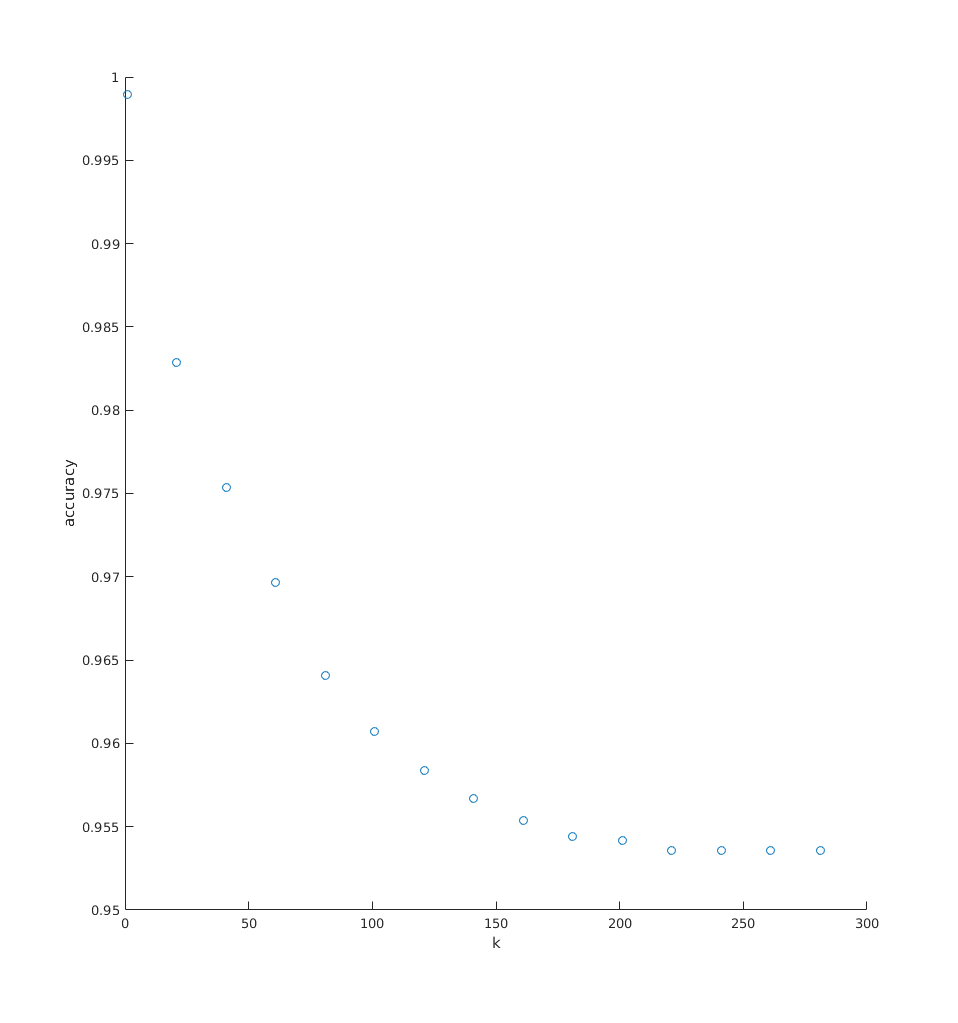
\includegraphics[width=\linewidth]{img/k_knn_accu.png}
\caption{Utilizando imágenes reducidas}
\end{subfigure}
\hfill
\begin{subfigure}[h]{0.62\linewidth}
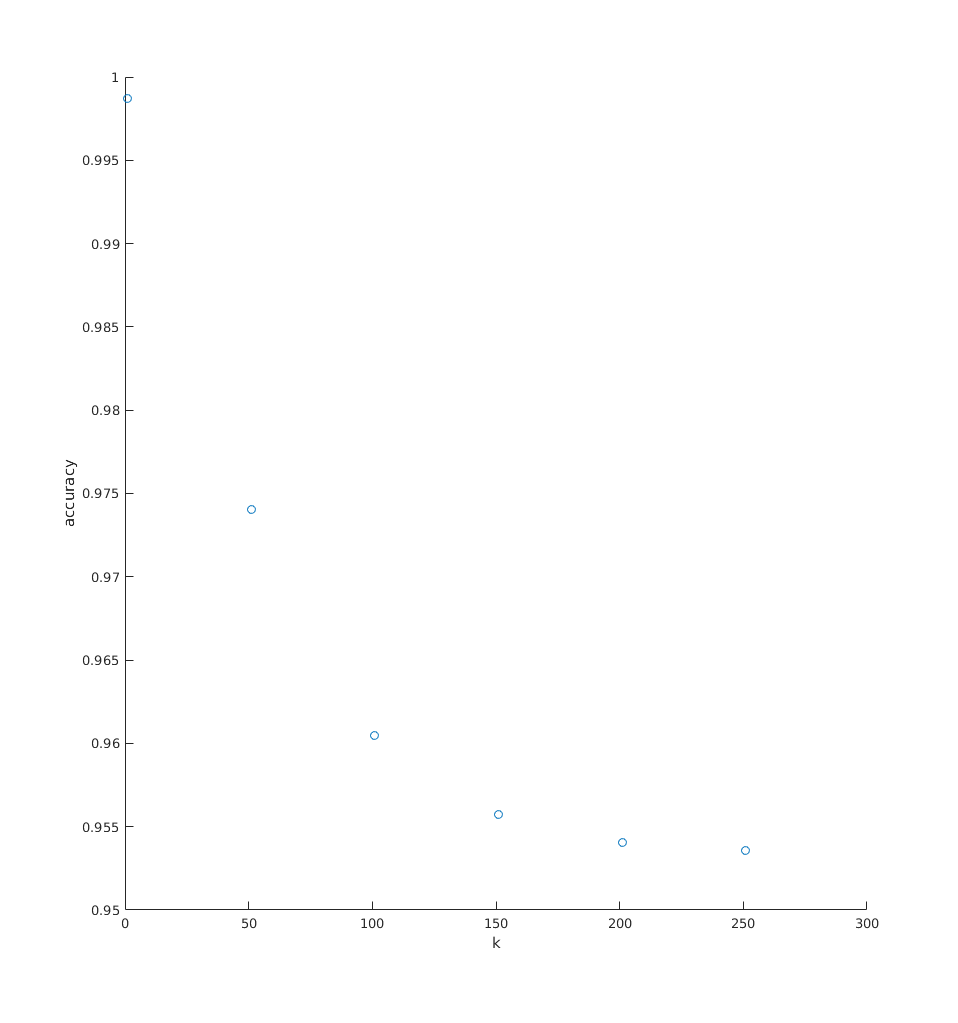
\includegraphics[width=\linewidth]{img/big_k_knn_accu.png}
\caption{Utilizando imágenes grandes}
\end{subfigure}%
\caption{K vs Accuracy con KNN sin PCA}
\end{figure}

En ambos casos obtenemos resultados similares, un Accuracy más grande a menor K, siendo K = 1 el valor óptimo, al menos en este caso.
%Dados los resultados, en este caso consideramos que utilizando un valor de K cercano a 10 obtenemos la mejor relación (dentro de nuestro set de tests).\newline
%Por un lado evitamos el problema que ocurre cuando K es demasiado grande y por otro, tomamos una cantidad de imágenes cercanas suficiente como para minimizar el impacto de algún outsider. Aun que cabe destacar que en este caso particular K = 1 tuvo un mejor comportamiento de lo que esperabamos, consideramos que sería arriesgado tomarlo como valor confiable con otros sets de imágenes.

%%%%%%%%%%%%%%%%%%%%%%%%%%%%%%%%%%%%%%%%%%%%%%%%%%%%%%%%%%%%%%%%%%%%%

\begin{figure}[H]
	\centering
	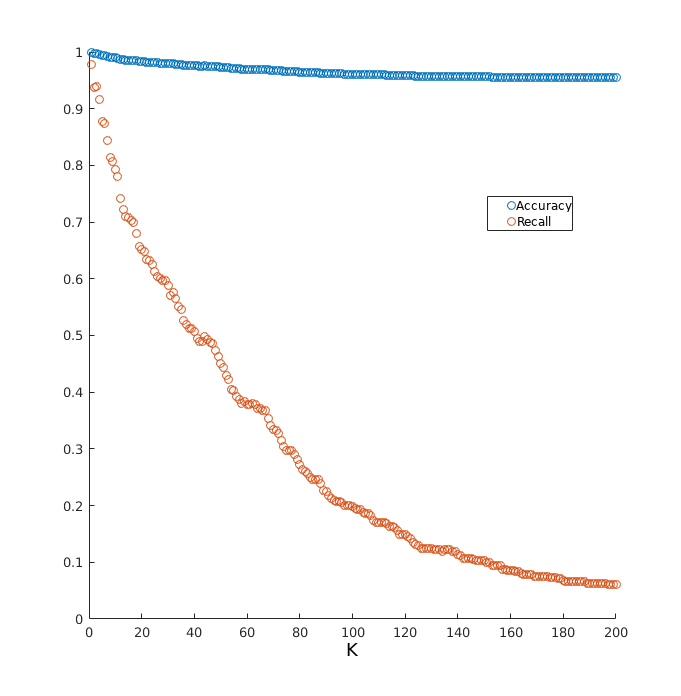
\includegraphics[width=0.8\textwidth]{img/Acc_recall_k_knn.png}
	\caption{Accuracy y Recall vs K (sin PCA)}
	\label{fig: Accuracy y Recall vs K (sin PCA)}
\end{figure}

En este gráfico encontramos algo similar al anterior, si bien se nota un descenso en Accuracy a medida que aumenta K, con el cambio de escala se puede apreciar que el mismo es muy leve.
Por el contrario, sí encontramos que Recall disminuye considerablemente a medida que K crece. En este caso es esta métrica la que nos da más elementos para concluir que K = 1 es la mejor opción.


%%%%%%%%%%%%%%%%%%%%%%%%%%%%%%%%%%%%%%%%%%%%%%%%%%%%%%%%%%%%%%%%%%%%%


%%%%%%%%%%%%%%%%%%%%%%%%%%%%%%%%%%%%%%%%%%%%%%%%%%%%%%%%%%%%%%%%%%%%%
%\begin{figure}[H]
%	\centering	
%	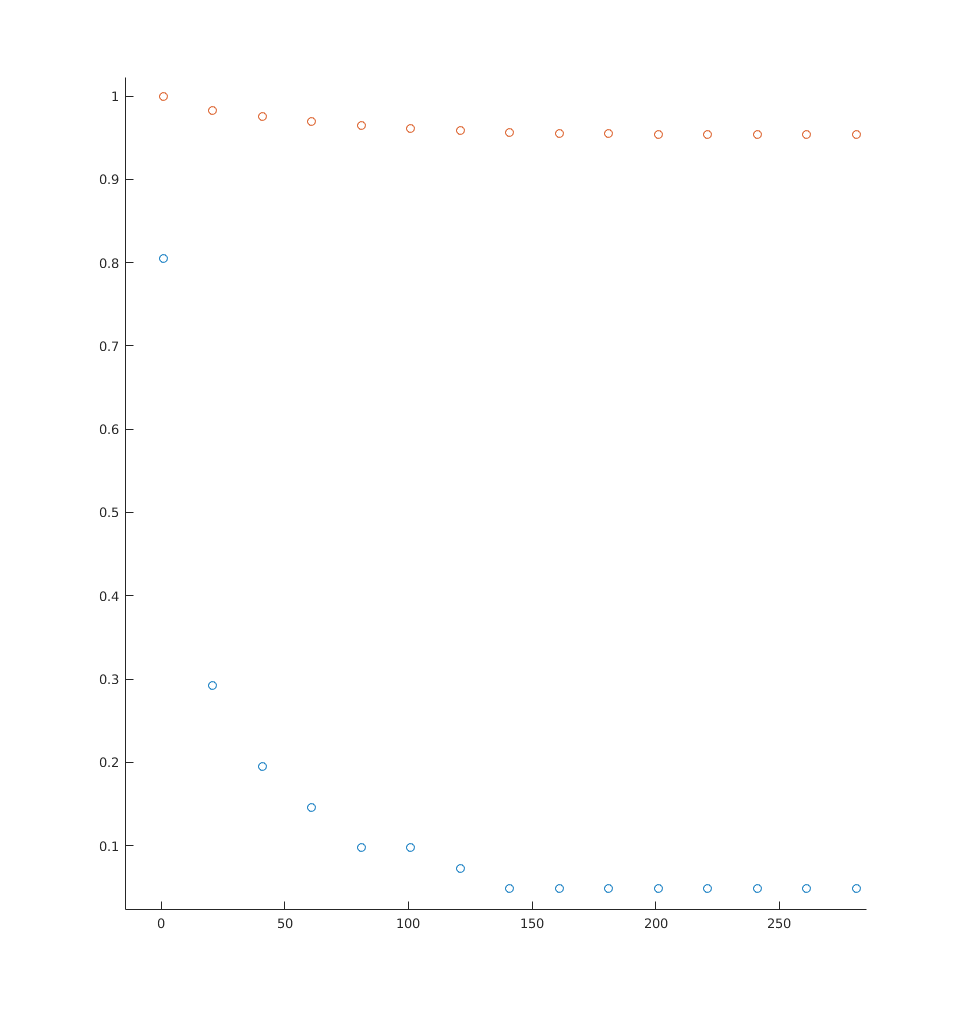
\includegraphics[width=0.8\textwidth]{img/acu_pre.png}
%	\caption{Accuracy y Precision vs K}
%	\label{fig: Accuracy y Precision vs K con KNN}
%\end{figure}

%En este experimento estudiamos cómo es que la cantidad de vecinos cercanos afecta a las métricas Accuracy y Recall.
%
%

%Lo que encontramos no fue muy distinto de lo esperado. En la figura anterior vimos la forma en la que Accuracy variaba en función de la cantidad de vecinos cercanos. Al cambiar la escala, observamos que la variación es bastante leve, pero como explicamos, por ejemplo elegir un K = 250 definitivamente no es una buena elección.
%
%Para tener un sistema robusto necesitamos un valor de (la métrica) recall relativamente alto. Luego en función de lo que nos indica el gráfico nuevamente un valor cercano a K = 1 nos parece adecuado.
%%%%%%%%%%%%%%%%%%%%%%%%%%%%%%%%%%%%%%%%%%%%%%%%%%%%%%%%%%%%%%%%%%%%%
\begin{figure}[H]
\begin{subfigure}[h]{0.62\linewidth}
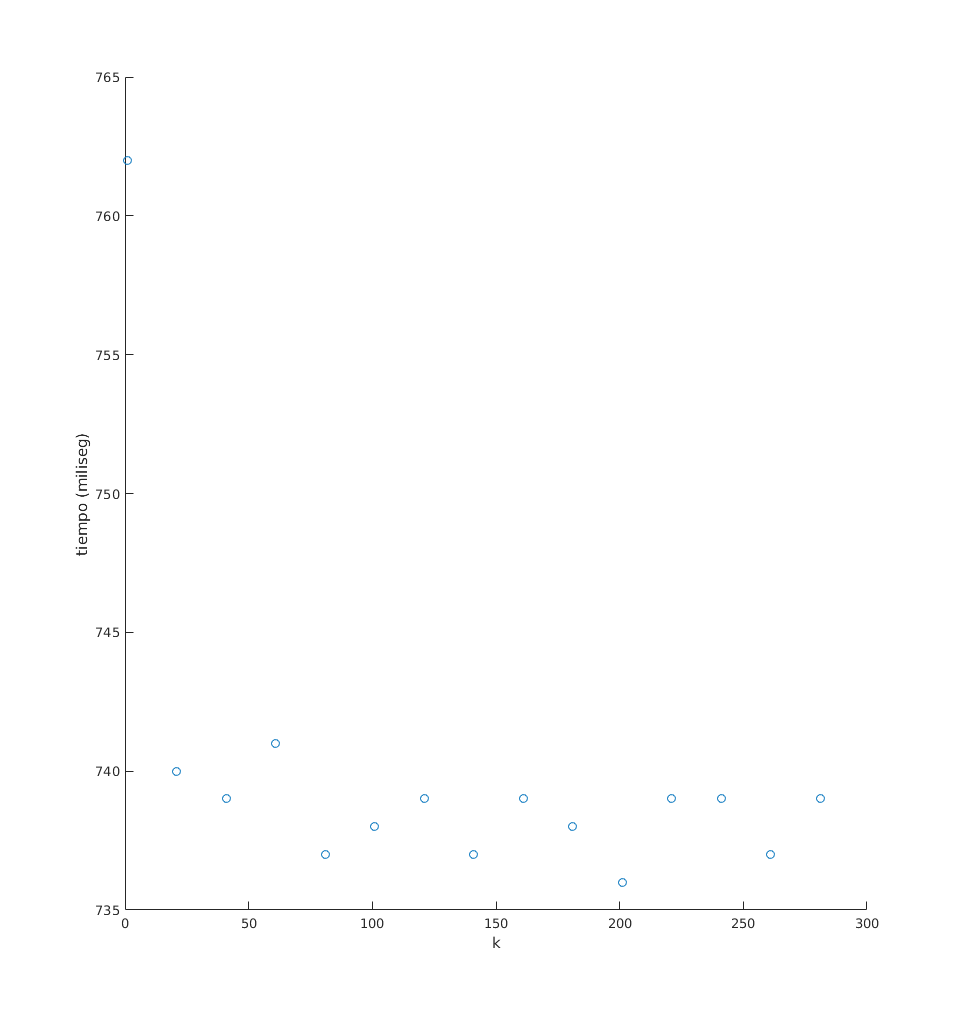
\includegraphics[width=\linewidth]{img/k_knn_tiempo.png}
\caption{Utilizando imágenes reducidas}
\end{subfigure}
\hfill
\begin{subfigure}[h]{0.62\linewidth}
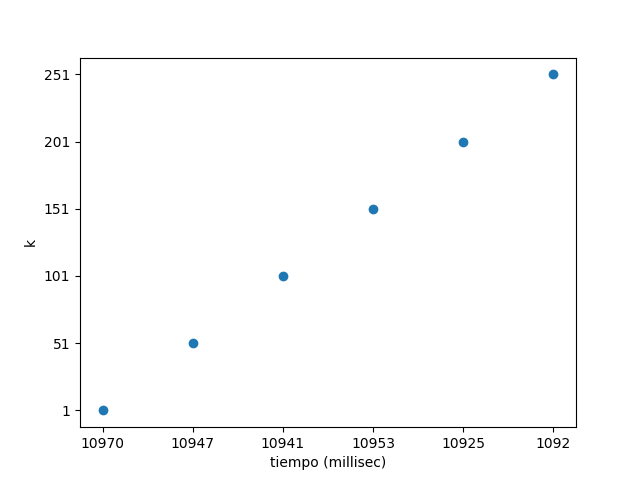
\includegraphics[width=\linewidth]{img/big_k_knn_tiempo.png}
\caption{Utilizando imágenes grandes}
\end{subfigure}%
\caption{Tiempo vs K con KNN sin PCA}
\end{figure}


En este caso no logramos identificar ningún patrón evidente. Si bien en el segundo gráfico se observan algúnas diferencias, en realidad representan pequeñas variaciones en el tiempo de ejecución que no consideramos relevantes.
Esto nos parece razonable, dado que por la forma de nuestra implementación calculamos la distancia con cada una de las imágenes y elegir un K mayor implica muy pocos cálculos adicionales.
%%%%%%%%%%%%%%%%%%%%%%%%%%%%%%%%%%%%%%%%%%%%%%%%%%%%%%%%%%%%%%%%%%%%%


\subsubsection*{Conclusiones del test}
Dados los resultados resulta evidente que cuánto más chico el K mejor se comportan nuestras métricas, luego concluímos que K = 1 es el valor óptimo.
Esto tiene sentido, sin embargo en caso de tener que implementar este problema en la vida real creemos que nos encontraríamos con outliers que pueden afectar el resultado, ya que con un solo vecino cercano tenemos un sistema poco robusto, por lo que elegiríamos un K un poco más grande pero cercano a 1.

%%%%%%%%%%%%%%%%%%%%%%%%%%%%%%%%%%%%%%%%%%%%%%%%%%%%%%%%%%%%%%%%%%%%%
\subsubsection*{Test con KNN + PCA}
Aquí evaluamos cómo se comporta nuestra implementación con PCA, para eso vamos a repetir los tests anteriores pero esta vez utilizando KNN+PCA.
De acuerdo a lo concluído de los tests anteriores inferimos que utilizar K = 1 o algún valor cercano sería lo mejor. 



%%%%%%%%%%%%%%%%%%%%%%%%%%%%%%%%%%%%%%%%%%%%%%%%%%%%%%%%%%%%%%%%%%%%%
\begin{figure}[H]
	\centering
	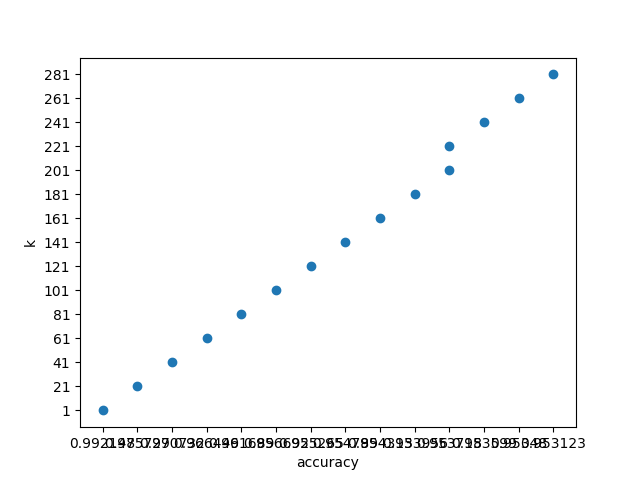
\includegraphics[width=0.8\textwidth]{img/k_pca_accu.png}
	\caption{Accuracy vs K con KNN + PCA}
	\label{fig:K vs Accuracy con KNN + PCA}
\end{figure}

En este caso observamos una estrecha relación entre cuántos vecinos cercanos tomamos y el Accuracy.
Nuevamente K = 1 parece ser el valor óptimo.

%%%%%%%%%%%%%%%%%%%%%%%%%%%%%%%%%%%%%%%%%%%%%%%%%%%%%%%%%%%%%%%%%%%%%

\begin{figure}[H]
\begin{subfigure}[h]{0.62\linewidth}
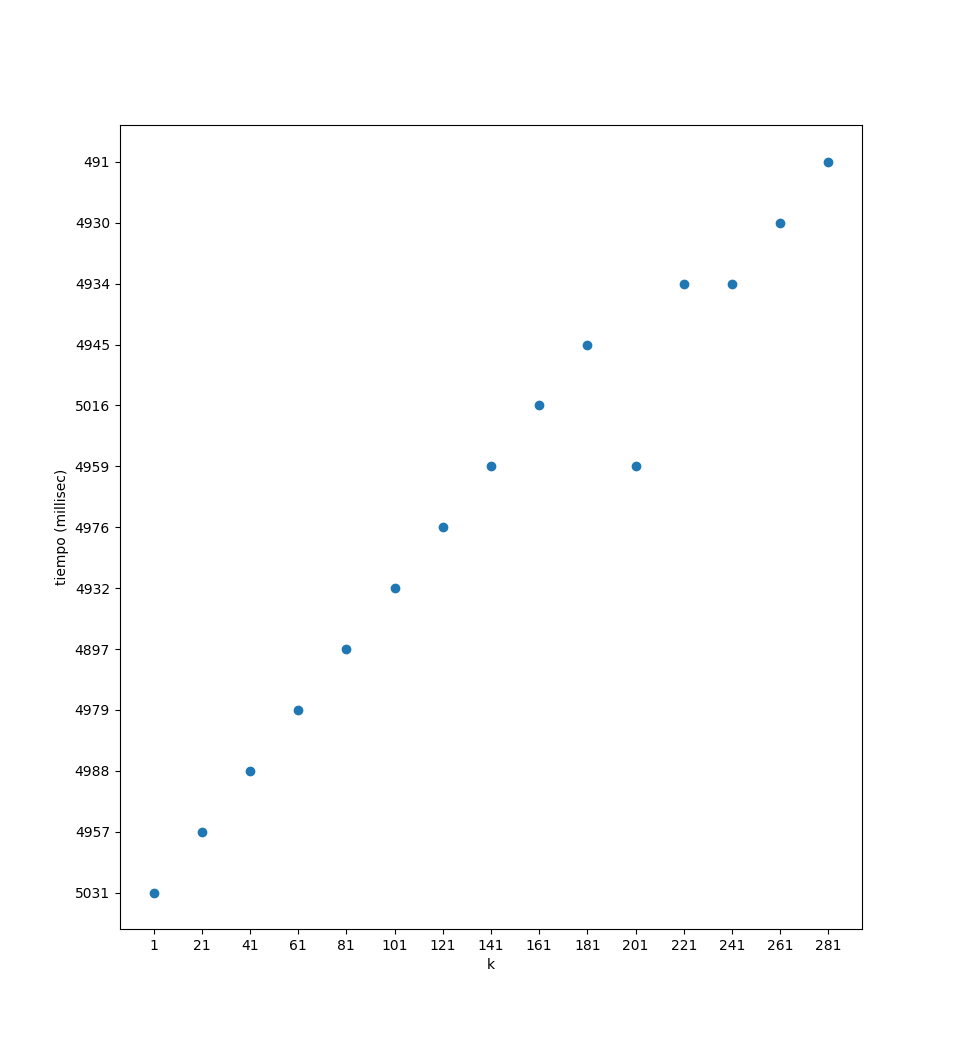
\includegraphics[width=\linewidth]{img/k_pca_tiempo.png}
\caption{Utilizando imágenes reducidas}
\end{subfigure}
\hfill
\begin{subfigure}[h]{0.62\linewidth}
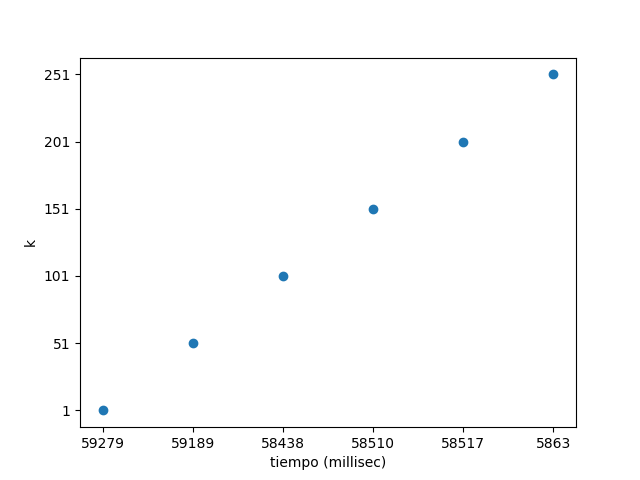
\includegraphics[width=\linewidth]{img/big_k_pca_tiempo.png}
\caption{Utilizando imágenes grandes}
\end{subfigure}%
\caption{Tiempo vs. K con KNN+PCA}
\end{figure}
Este caso es muy similar al visto sin PCA (Figura 3), no notamos diferencias relevantes.

Nótese que al calcular el tiempo incluimos desde el principio hasta el final del algoritmo. Para apreciar mejor la función de PCA tendríamos que haber calculado el tiempo del reconocimiento sin contar el cálculo de PCA. Este fue un hecho que notamos una vez terminada la experimentación pero sería un experimento interesante, que dejaremos para un futuro.\newline
Sin embargo vimos que PCA funciona correctamente en cuanto a nuestras métricas y por nuestra implementación, al trabajar con una matriz más chica obtendríamos una reducción en el tiempo de ejecución (tal como observamos al probar KNN sin PCA con el set de imágenes chico y el gránde), con esto podemos deducir que el reconocimiento una vez aplicado PCA tarda menos y a la vez sigue siendo efectivo.

%%%%%%%%%%%%%%%%%%%%%%%%%%%%%%%%%%%%%%%%%%%%%%%%%%%%%%%%%%%%%%%%%%%%%

\begin{figure}[H]
\begin{subfigure}[h]{0.62\linewidth}
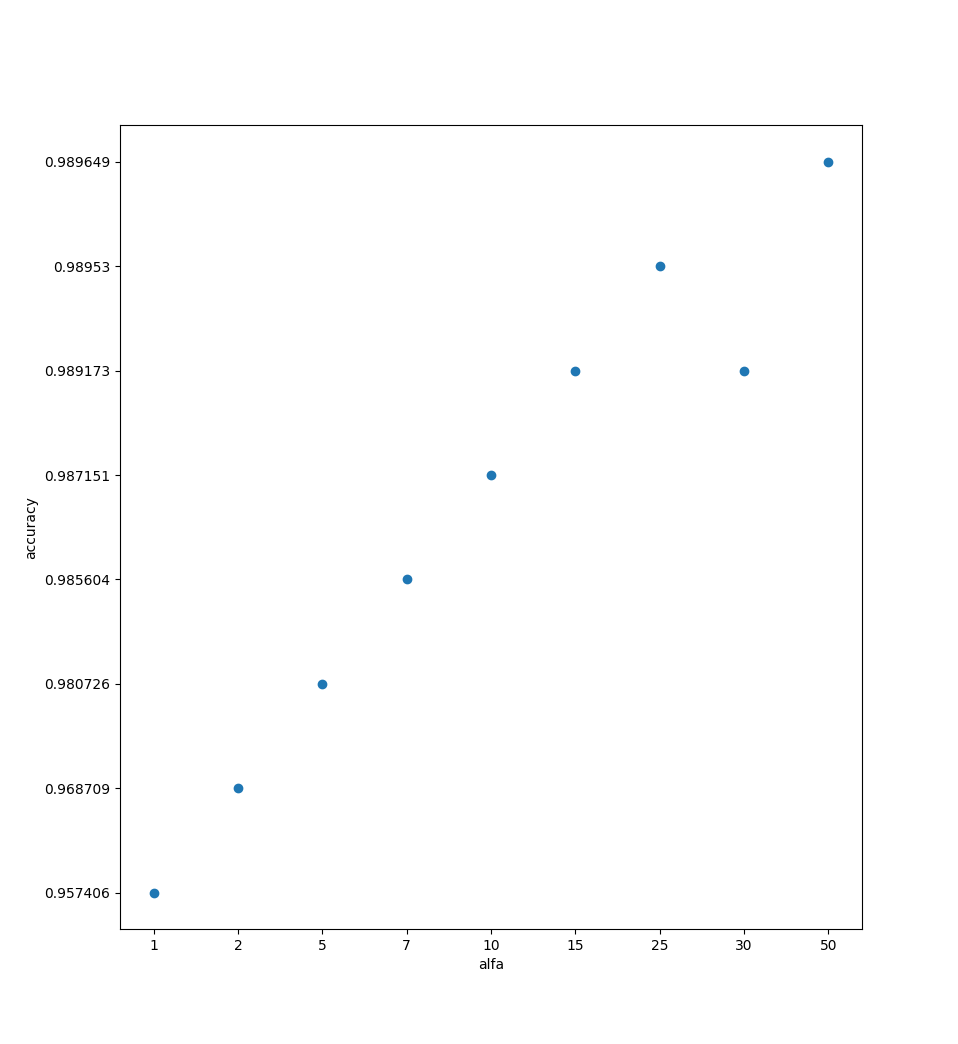
\includegraphics[width=\linewidth]{img/alfa_pca_accu.png}
\caption{Utilizando imágenes reducidas}
\end{subfigure}
\hfill
\begin{subfigure}[h]{0.62\linewidth}
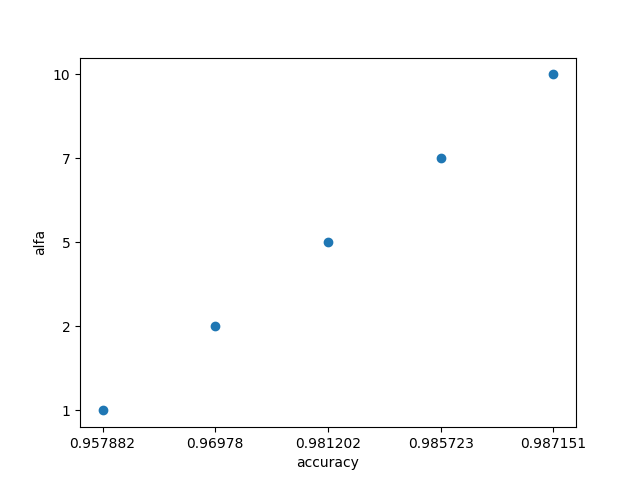
\includegraphics[width=\linewidth]{img/big_alfa_pca_accu.png}
\caption{Utilizando imágenes grandes}
\end{subfigure}%
\caption{Accuracy vs $\alpha$ con KNN+PCA}
\end{figure}

En este caso podemos observar una relación entre las dos variables, a medida que el $\alpha$ aumenta vemos como también lo hace nuestro accuracy.
Como expresamos anteriormente, debido al funcionamiento de PCA esperábamos que a mayor $\alpha$, obtendríamos una mejor reconstrucción y por lo tanto mejores resultados (en todas nuestras métricas en general).

Pero a su vez vimos que un $\alpha$ muy elevado resultaría en un aumento del tiempo de ejecución, no obstante en este gráfico vemos como las diferencias entre accuracy son cada vez menores, es decir como disminuye la pendiente (por ejemplo entre $\alpha$ = 10 y $\alpha$ = 50).

En base a los resultados obtenidos concluimos que un valor de $\alpha$ cercano a 10 nos daría un buen balance entre la cantidad de componentes principales y la efectividad (la cuál disminuye un poco, pero a cambio trabajamos con imágenes mucho más chicas).

Se puede ver en el gráfico a) que el valor máximo probado es $\alpha$ = 50 mientras que en el gráfico b) es $\alpha$ = 10. Esto se debe a que al trabajar en b) con imágenes más grandes requería mucho tiempo de ejecución ya que en los tests se realiza el preprocesamiento de las imágenes en cada corrida, por esto es que probamos solo hasta ese valor, donde igualmente podemos notar la forma del gráfico.

%%%%%%%%%%%%%%%%%%%%%%%%%%%%%%%%%%%%%%%%%%%%%%%%%%%%%%%%%%%%%%%%%%%%%
\begin{figure}[H]
\begin{subfigure}[h]{0.62\linewidth}
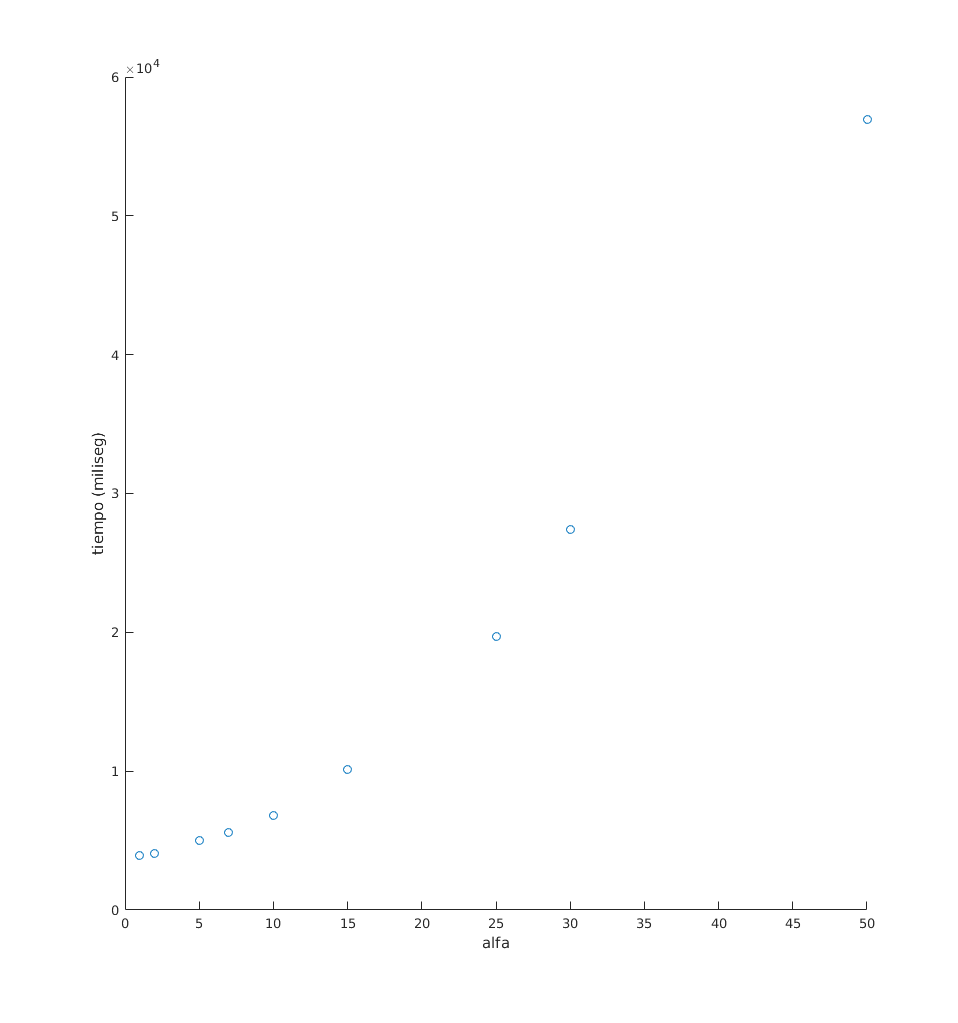
\includegraphics[width=\linewidth]{img/alfa_pca_tiempo.png}
\caption{Utilizando imágenes reducidas}
\end{subfigure}
\hfill
\begin{subfigure}[h]{0.62\linewidth}
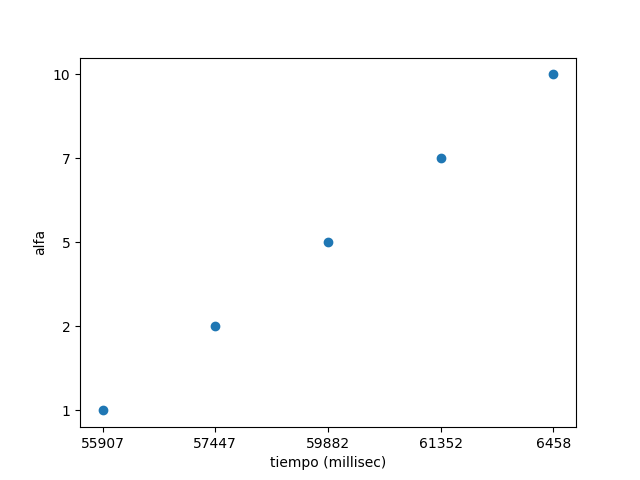
\includegraphics[width=\linewidth]{img/big_alfa_pca_tiempo.png}
\caption{Utilizando imágenes grandes}
\end{subfigure}%
\caption{Tiempo vs $\alpha$ con KNN+PCA}
\end{figure}

Tal como esperábamos vemos que a medida que el $\alpha$ aumenta (es decir, cuantas más componentes principales tengamos), el tiempo de ejecución también lo hace.

Luego, en línea con los resultados de los gráficos anteriores (Accuracy vs $\alpha$) podemos volver a afirmar que un $\alpha$ cercano a 10 sería un buen balance. En a) notamos que si tomáramos $\alpha$ = 30, tardaría aproximadamente el triple y no obtendríamos una mejora en el accuracy que valga la pena.
%%%%%%%%%%%%%%%%%%%%%%%%%%%%%%%%%%%%%%%%%%%%%%%%%%%%%%%%%%%%%%%%%%%%%
\begin{figure}[H]
	\centering
	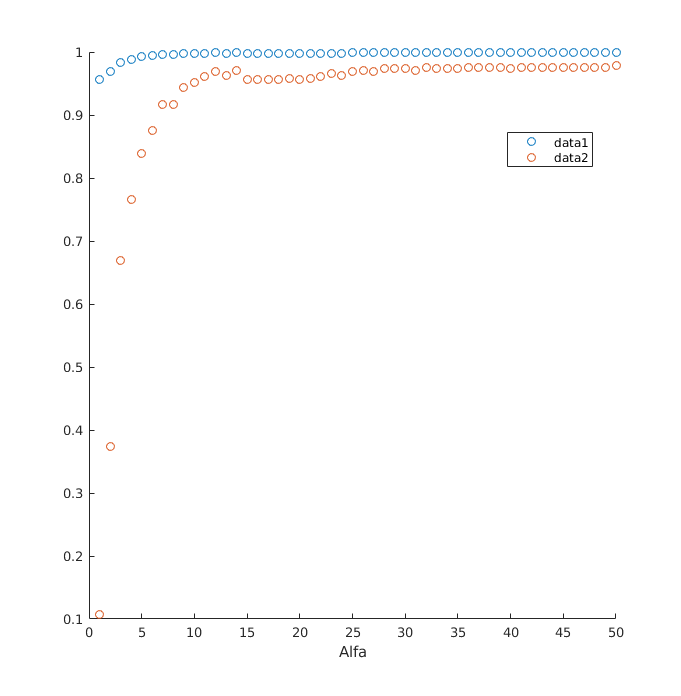
\includegraphics[width=0.8\textwidth]{img/Acc_recall_alfa_pca.png}
	\caption{Accuracy y Recall vs Alfa (con PCA)}
	\label{fig: Accuracy y Recall vs Alfa (con PCA)}
\end{figure}

En este caso al evaluar también recall observamos algo similar, a partir de 10 obtenemos un valor aceptable de esta métrica.
%%%%%%%%%%%%%%%%%%%%%%%%%%%%%%%%%%%%%%%%%%%%%%%%%%%%%%%%%%%%%%%%%%%%%

\begin{figure}[H]
	\centering
	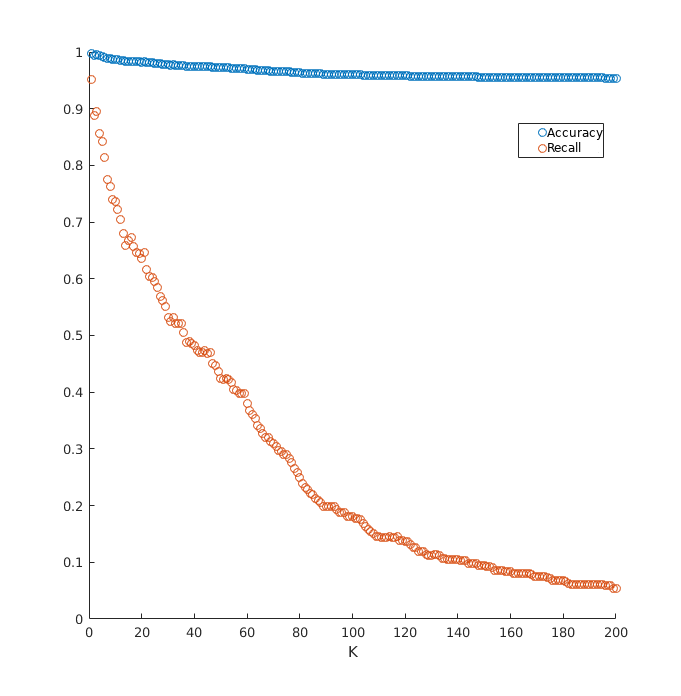
\includegraphics[width=0.8\textwidth]{img/Acc_recall_k_pca.png}
	\caption{Accuracy y Recall vs K (con PCA)}
	\label{fig: Accuracy y Recall vs K (con PCA)}
\end{figure}
Observamos que el resultado es realmente similar al del mismo test llevado a cabo sin PCA, luego por los mismos argumentos utilizados en el caso mencionado decimos que K = 1 es el mejor valor.
También podríamos agregar que el hecho de obtener resultados muy similares al test sin PCA habla bien del funcionamiento de PCA (con $\alpha$ = 10) que obtiene una buena tasa de reconocimiento con muy pocas componentes (lo que equivale a un gran ahorro de espacio).
%%%%%%%%%%%%%%%%%%%%%%%%%%%%%%%%%%%%%%%%%%%%%%%%%%%%%%%%%%%%%%%%%%%%%

Llegamos a la conclusión de que utilizando un valor de K cercano a 10 obtenemos la mejor relación (dentro de nuestro set de tests).
Por un lado evitamos el problema que ocurre cuando K es demasiado grande y por otro, tomamos una cantidad de imágenes cercanas suficiente como para minimizar el impacto de algún outsider.




\section{Discusión}
Las expectativas que teníamos respecto de las pruebas usando solo KNN en comparación a KNN + PCA era que la segunda iba a dar mejores resultados en cuanto a las métricas de reconocimiento, sin embargo esto no fue así, lo que sí se logra usando PCA es trabajar con matrices más chicas, lo cual es útil si se trabaja con una base de datos con imágenes grandes o con muchas imágenes.
Con respecto a los tiempos tal como esperábamos PCA resulta lento en el procesamiento de la base de datos de entrenamiento sobre todo cuando se agregan muchas componentes principales. También suponíamos que las primeras componentes principales iban a influir más en tener buenos resultados de reconocimiento. Esto efectivamente fue así y lo usamos al diseñar los casos de test usando $\alpha$ más próximos en los valores pequeños y espaciándolos en valores más altos.
Una de las cosas que suponíamos es que usando un K más alto en KNN iba a funcionar mejor, pero esto no fue así, dando mejores métricas para K más chicos.
Los tiempos de ejecución fue una de las cuestiones que tuvimos en cuenta a a hora de diseñar los casos de pruebafundamentalmente en las corridas que usan PCA.

\section{Conclusiones}
\subsubsection*{Conclusiones}


\section{Apendices}
\subsubsection*{Apéndices}


\section{Referencias}
\subsubsection*{Referencias}

 

\end{document}
